\documentclass[a4paper]{report}
\usepackage[T1]{fontenc}
\usepackage[french]{babel}
\usepackage[utf8x]{inputenc}
\usepackage{amsmath}
\usepackage{eurosym}
\usepackage{float}
\usepackage{graphicx}
\usepackage[colorinlistoftodos]{todonotes}
\usepackage{placeins}
\usepackage{verbatim}
\usepackage{fmtcount}
\usepackage{array}
\usepackage[toc,page]{appendix} 
\renewcommand{\arraystretch}{1.25}

\usepackage{tabularx}
\newcounter{cptspec}
\setcounter{cptspec}{0}
 
\title{INSA de Rennes \\ Quatrième année Informatique \\ \bigskip \hrule \bigskip Rapport de planification \\ \bigskip Projet VaR \bigskip \hrule}

\author{Benjamin \bsc{Bouguet} - Damien \bsc{Carduner} \\Paul \bsc{Chaignon} - Eric \bsc{Chauty} - Xavier \bsc{Fraboulet} \\ Clément \bsc{Gautrais} - Ulysse \bsc{Goarant} \\ ~~\\
Hamdi \bsc{Raissi} - Quentin \bsc{Giai Gianetto}}


\date{Décembre 2013}

\begin{document}
\maketitle

\thispagestyle{empty}
\newpage

~~
\thispagestyle{empty}
\newpage


\tableofcontents
\newpage


\chapter{Introduction}
Dans le milieu de la finance, les prises de décisions liées aux investissements sont en grande partie motivées par une estimation des risques associés. De plus, l'établissement des accords de Bâle dont le troisième et dernier a été publié fin 2010, obligent les banques à s'organiser dans ce sens. En effet, il s'agit d'accords de réglementations bancaires qui visent à garantir un niveau minimum de capitaux afin d'assurer la solidité financière des banques. Afin d'être en règle vis-à-vis de ces accords, des outils de gestion de risque, tels que la Value-at-Risk (VaR) peuvent être utilisés. La VaR correspond à la perte associée à un actif qu'il est probable de ne pas excéder pour un niveau de confiance et un horizon de temps donnés. Par exemple, une banque peut déterminer une VaR de 100,000~€ pour un niveau de confiance de 5\% et un horizon de temps d'un mois. Cela signifie qu'il y a une probabilité de 5\% de perdre plus de 100,000~€ d'ici un mois. 

Notre logiciel sera justement un outil d'aide à la décision qui permettra de calculer la VaR  par diverses méthodes statistiques. Il proposera également un ensemble de tests, comparaisons, tableaux récapitulatifs et backtesting\footnote{Le backtesting ou test rétroactif de validité consiste à tester la pertinence d'une modélisation ou d'une stratégie en s'appuyant sur un large ensemble de données historiques réelles.} entre les différentes méthodes statistiques. Avec cette multitude d'outils, les financiers seront en mesure de travailler sur leurs portefeuilles\footnote{Un portefeuille est une composition de plusieurs actifs financiers (actions, obligations, matières premières).} aisément, au moyen d’une interface simple, intuitive et ergonomique, pensée pour l'utilisation au quotidien.

Le rapport de spécification fonctionnelle détaillait nos choix d’implémentation. Ce rapport de planification qui est le complément direct du précédent, précise la planification associée à nos choix. Dans un premier temps, nous allons indiquer des informations de base telles que les dates clés ou les outils de travail. Dans un second temps, nous décrirons la planification de chaque partie décrite dans le rapport de spécification fonctionnelle. Enfin, nous nous appuierons sur les coûts estimés en heures des différentes parties et leurs dépendances pour présenter un diagramme de GANTT résumant notre planification jusqu’à la fin du projet.

\chapter{Informations de base}
\section{Dates clés}
Dans cette partie, nous décrivons les dates clés présentes à la suite du travail de planification. L'étape principale suivante correspond à la phase de conception. Elle s'achève le 13 février. Son achèvement est nécessaire avant l'amorce de la phase de développement. Cependant, nous envisageons la prise en main de certains outils tels que Qt et l'interface avec R\footnote{R est un logiciel libre de traitement des données et d'analyse statistiques.} avant le début de la phase de développement afin d'être plus efficace lors de cette dernière.
Nous créerons ensuite pour le 3 avril un document HTML en français et en anglais décrivant notre projet.
Nous rendrons le 25 mai le rapport final qui décrit les phases de tests, les rectificatifs apportés aux rapports de spécification et de conception, l'état de finalisation du projet ainsi qu'un bilan de la planification. Enfin, nous produirons pour le 28 mai une documentation en ligne du code développé.

\section{Ressources humaines}
Notre planification des tâches prend en compte la réduction des ressources humaines à quatre personnes lors du second semestre.

\section{Temps de travail}
Le tableau \ref{fig:travail} récapitule le nombre d'heures de travail par semaine pour une personne.

\begin{table}[H]
\centering
  \begin{tabularx}{0.8\textwidth}{| X | c | c |}
    \hline
	Type de semaine & Nombre & Temps de travail \\
    \hline
    Semaine normale & 13 & 7h \\
    \hline
    Semaine de vacances & 1 & 25h \\
    \hline
    Semaine de partiels/révisions & 3 & 3h \\
    \hline
    Semaine de projet & 2 & 40h \\
    \hline
  \end{tabularx}
  \caption{Temps de travail}
  \label{fig:travail}
\end{table}


\chapter{Étapes du projet}


\section{Conception}
La phase de conception intervient après les phases de pré-étude et de spécification. Cette phase du projet précède nécessairement les phases de développement et de tests. Sa durée totale est estimée à 40 heures. Une partie importante du rapport de conception consistera en la création de diagrammes UML. Les diagrammes de classes et les diagrammes d'interactions seront complémentaires et permettont de faciliter et de rendre plus fluide la phase de développement. De même les diagrammes d'activité permettont de déterminer la succession des actions réalisées par une personne sur le logiciel.

\begin{table}[H]
\centering
  \begin{tabularx}{0.8\textwidth}{| X | c |}
    \hline
	Tâches & Charges \\
    \hline
     Diagrammes de classes & 10h \\
     Diagrammes d'activité & 5h \\
     Diagrammes d'interactions & 10h \\
     %Diagramme de classe & 25h
     Rédaction du rapport de conception &  15h\\
    \hline
  \end{tabularx}
  \caption{Durées des tâches liées à la conception}
\end{table}


\section{Développement}
Une fois que le rapport de conception sera terminé, nous pourrons commencer le dévelopement des différents modules du logiciel. Dans la suite de cette partie, nous allons décrire les tâches associées.

\subsection{Gestion des données}
Le calcul de la Value-At-Risk s'effectuant sur des données financières, il est nécessaire de commencer par implémenter la gestion des données.

\subsubsection{Actifs}
Les actifs constituent les éléments de base des données manipulées dans le logiciel. La première étape sera donc d'implémenter le modèle obtenu lors de la phase de conception. C'est à dire de créer une classe et les méthodes associées.

De plus, puisque ces données proviennent de sources externes comme Yahoo Finance ou Bloomberg, il est important de pouvoir importer ces fichiers. Deux formats de fichiers, CSV et XLSX, seront pris en charge par le logiciel ce qui entrainera un travail important sur la partie importation.

\begin{table}[H]
\centering
  \begin{tabularx}{0.8\textwidth}{| X | c |}
    \hline
	Tâches & Charges \\
    \hline
    Modélisation des actifs dans le logiciel & 10h \\
    Importation des actifs & 20h \\
    Exportation des actifs & 10h \\
    \hline
  \end{tabularx}
  \caption{Durées des tâches liées aux actifs}
\end{table}


\subsubsection{Portefeuilles}
Les portefeuilles sont constitués d'une composition d'actifs. Il est donc nécessaire d'avoir préalablement implémenté la gestion des actifs avant d'envisager l'implémentation de la gestion des portefeuilles.
De plus, nous avons estimé qu'importer et exporter des portefeuilles constitueront des tâches importantes en terme de charge de travail.

\begin{table}[H]
\centering
  \begin{tabularx}{0.8\textwidth}{| X | c |}
    \hline
	Tâches & Charges \\
    \hline
     Modélisation des portefeuilles dans le logiciel &  20h\\
     Importer un portefeuille &  15h\\
     Exporter un portefeuille &  10h\\
    \hline
  \end{tabularx}
  \caption{Durées des tâches liées aux portefeuilles}
\end{table}


\subsection{Calculs}
Les fonctionnalités de calcul contiennent principalement le calcul de la Value-at-Risk selon différentes méthodes. Pour calculer cette dernière, nous allons utiliser le logiciel de statistiques R. Il faudra donc dans un premier temps, interfacer notre logiciel avec R. Une fois que l'appel de scripts R depuis notre application sera possible, nous pourrons réaliser les différentes méthodes de calcul de la Value-at-Risk (VaR).

La modélisation GARCH se fera via un simple appel de fonction R. Le développement de la méthode bootstrap sera ce qui prendra le plus de temps dans la modélisation GARCH.

Le calcul par la méthode historique sera assez rapide car il consiste simplement à prendre un quantile de la distribution des rendements, ce qui est rapidement faisable avec R.

En utilisant la méthode Riskmetrics, le calcul de la VaR sera assez rapide car les tâches sont similaires à celles de la modélisation GARCH.

Les tests de corrélation nous ont été fournis sous forme de scripts R par notre encadrant. Il nous faudra d'abord les tester (ce qui correspond à la tâche de test des scripts externes) puis les appeler via R. Comme cet appel est différent d'une simple utilisation de R, nous avons prévu une durée un peu plus longue.

Enfin, les calculs statistiques se résumeront à de simples appels à des fonctions fournies par R. C'est pourquoi cette tâche est relativement courte. 

Nous voyons bien ici l'importance de la première tâche (interfaçage avec R) pour le bon déroulement des tâches suivantes. Comme l'interfaçage semble être compliqué, nous avons donc choisi d'affecter une durée assez longue pour cette tâche.

\begin{table}[H]
\centering
  \begin{tabularx}{0.8\textwidth}{| X | c |}
    \hline
	Tâches & Charges \\
    \hline
    Interfaçage avec R &  20h \\
    Modélisation GARCH &  15h \\
    Méthode historique &  5h \\
    Méthode Riskmetrics &  10h \\
    Tests de corrélation &  10h \\
    Tests scripts externes R & 5h \\
    Calculs statistiques &  5h \\
    \hline
  \end{tabularx}
  \caption{Durées des tâches liées aux calculs}
\end{table}

\subsection{Backtesting}
Le développement du backtesting nécessite préalablement le fonctionnement du calcul de la VaR selon les différentes méthodes de calcul, à savoir la méthode historique, la méthode Riskmetrics et la méthode basée sur les modèles GARCH.

\begin{table}[H]
\centering
  \begin{tabularx}{0.8\textwidth}{| X | c |}
    \hline
	Tâches & Charges \\
    \hline
    Backtesting &  30h \\
    \hline
  \end{tabularx}
  \caption{Durées des tâches liées au backtesting}
\end{table}


\subsection{Rapports}
De manière générale, les rapports résument les informations générées par les autres modules du logiciel. Il n'est cependant pas nécessaire que le module correspondant au rapport à générer soit d'abord implémenté. Ceci permet le développement en parallèle du module de la génération des rapports et des modules correspondants d'où sont extraites les données.

\begin{table}[H]
\centering
  \begin{tabularx}{0.8\textwidth}{| X | c |}
    \hline
	Tâches & Charges \\
    \hline
    Rapport au format \emph{DOCX} &  10h \\
    Rapport au format \emph{PDF} &  10h \\
    Rapport du calcul de la VaR & 5h \\
    Rapport de statistiques générales & 5h \\
    Rapport de matrice de covariance & 5h \\
    Rapport de backtesting & 5h \\
    \hline
  \end{tabularx}
  \caption{Durées des tâches liées aux rapports}
\end{table}


\subsection{Graphiques}
Les graphiques nécessitent principalement l'implémentation de la gestion des données. L'implémentation des matrices de corrélation nécessite de plus celle des calculs correspondants.

\begin{table}[H]
\centering
  \begin{tabularx}{0.8\textwidth}{| X | c |}
    \hline
	Tâches & Charges \\
    \hline
    Matrice de corrélation &  15h \\
    Histogramme &  15h \\
    \hline
  \end{tabularx}
  \caption{Durées des tâches liées aux graphiques}
\end{table}


\subsection{IHM}
L'IHM contient toutes les actions que l'utilisateur peut effectuer, les formulaires que l'utilisateur devra remplir ainsi que les éléments graphiques tels que les tableaux. La durée des tâches comprend aussi la gestion des messages d'erreurs ainsi que leur affichage dans l'IHM. Il sera possible de démarrer le développement de l'IHM en parallèle de celui des autres modules.

\begin{table}[H]
\centering
  \begin{tabularx}{0.8\textwidth}{| X | c |}
    \hline
	Tâches & Charges \\
    \hline
    Exporter des actifs & 5h\\
    Importer des actifs & 10h\\
    Backtesting & 5h\\
    Calcul de la VAR & 5h\\
    Ajouter/Modifier portefeuille & 10h\\
    Gestion des sessions & 10h\\
    Générer rapports & 5h\\
    Calculs statistiques & 5h\\
    Exporter un portefeuille & 10h\\
    Importer un portefeuille & 5h\\
    Supprimer un portefeuille & 5h\\
    Listing des portefeuilles & 10h \\
    Afficher le contenu d'un portefeuille & 10h \\
    Afficher les rapports d'un portefeuille & 5h \\
    \hline
  \end{tabularx}
  \caption{Durées des tâches liées à l'IHM}
\end{table}


\subsection{Session}
La gestion des sessions permet de sauvegarder l'ensemble du travail en cours et de le réimporter ultérieurement. Concrètement, les données et les calculs sont sauvegardés sur le disque et importés automatiquement au lancement d'une nouvelle session. Cette tâche nécessite que la gestion des actifs et des portefeuilles soit en partie déjà réalisée.


\begin{table}[H]
\centering
  \begin{tabularx}{0.8\textwidth}{| X | c |}
    \hline
	Tâches & Charges \\
    \hline
    Sauvegarde de la session &  10h \\
    Restaurer la session &  10h \\
    \hline
  \end{tabularx}
  \caption{Durées des tâches liées à la session}
\end{table}


\section{Tests}

Nous effectuerons des tests au fûr et à mesure du développement, et entièrement à la fin du projet. De plus, les tests unitaires de la gestion des données (et des algorithmes de calcul) seront écrits dès qu'une fonctionnalité (respectivement un algorithme) sera écrite. L'IHM étant plus difficile à tester automatiquement, nous ne pensons pas le faire. Cependant celle-ci sera testée (manuellement) au fûr et à mesure de son développement et entièrement à la fin du projet.


\begin{table}[H]
\centering
  \begin{tabularx}{0.8\textwidth}{| X | c |}
    \hline
	Tâches & Charges \\
    \hline
    Tests de la gestion des données & 20h \\
    Tests des calculs (modèle et VaR) & 20h \\
    Tests IHM & 20h \\
    \hline
  \end{tabularx}
  \caption{Durées des tâches liées aux tests}
\end{table}


\section{Documentations}

\subsection{Pages HTML}
La rédaction de pages HTML en anglais et en français constituera un moyen de décrire de manière synthétique notre projet.


\begin{table}[H]
\centering
  \begin{tabularx}{0.8\textwidth}{| X | c |}
    \hline
	Tâches & Charges \\
    \hline
    Rédaction des pages HTML & 5h\\
    \hline
  \end{tabularx}
  \caption{Durées des tâches liées aux pages HTML}
\end{table}


\subsection{Documentation en ligne}

L'ajout de commentaires dans notre code tout au long du projet nous permettra de générer une documentation claire pour le 28 mai.

\begin{table}[H]
\centering
  \begin{tabularx}{0.8\textwidth}{| X | c |}
    \hline
	Tâches & Charges \\
    \hline
    Rédaction de la documentation & 5h \\
    \hline
  \end{tabularx}
  \caption{Documentation en ligne}
\end{table}


\subsection{Rapport final et rapport de bilan de planification}

La rédaction du rapport final sera l'occasion de faire un bilan de notre projet. Il décrira les phases de tests, les rectificatifs apportés aux rapports de spécification et de conception, ainsi qu'un bilan de la planification.

\begin{table}[H]
\centering
  \begin{tabularx}{0.8\textwidth}{| X | c |}
    \hline
	Tâches & Charges \\
    \hline
    Compte rendu des phases de test & 20h \\
    Rectificatif des rapports précédents & 10h \\
    Bilan de la planification & 10h \\
    \hline
  \end{tabularx}
  \caption{Durées des tâches liées au rapport final}
\end{table}



\chapter{Diagramme de GANTT}

A partir de ces charges estimées nous pouvons maintenant créer le diagramme de GANTT. Ce dernier a été réalisé grâce au logiciel \emph{Microsoft Project}.

Le diagramme de la figure \ref{fig:gantt} permettra de déterminer à la fois si nos prévisions de charge de travail sont réalistes et également de connaître tout au long des phases de travail notre état d'avancement dans la réalisation du projet.


\vspace{0.5cm}

Le diagramme de taux d'utilisation de la figure \ref{fig:sample-graph} permet de constater que la charge de travail est bien répartie sur l'ensemble du projet. Seulement une semaine sera très légèrement surchargée.

Les derniers mois du projet sont moins chargés : en moyenne le taux d'utilisation par semaine des ressources est inférieur à 80\%. Cela permettra de compenser d'éventuels retards pris au cours des mois de février et de mars consacrés au développement et aux tests.

\begin{figure}[tb] 
\centering
\vspace*{-3cm}
 \makebox[\textwidth]{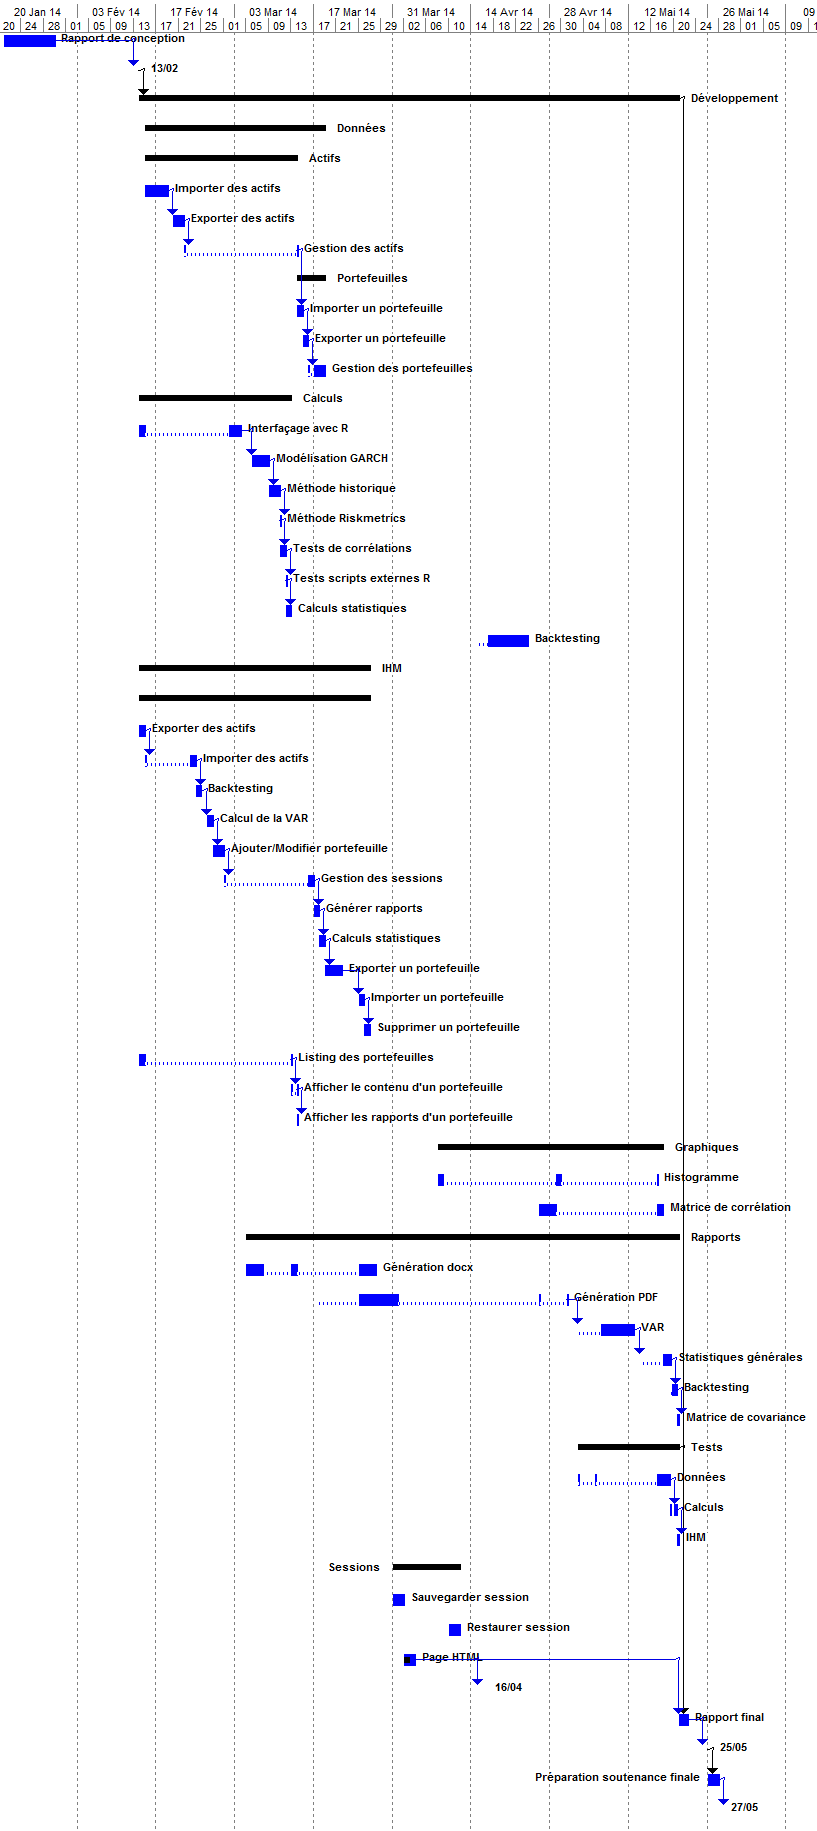
\includegraphics[width=0.5\paperwidth]{GANT.png}}
\caption{\label{fig:gantt}Diagramme de GANT}


\end{figure}

\begin{figure}
\centering
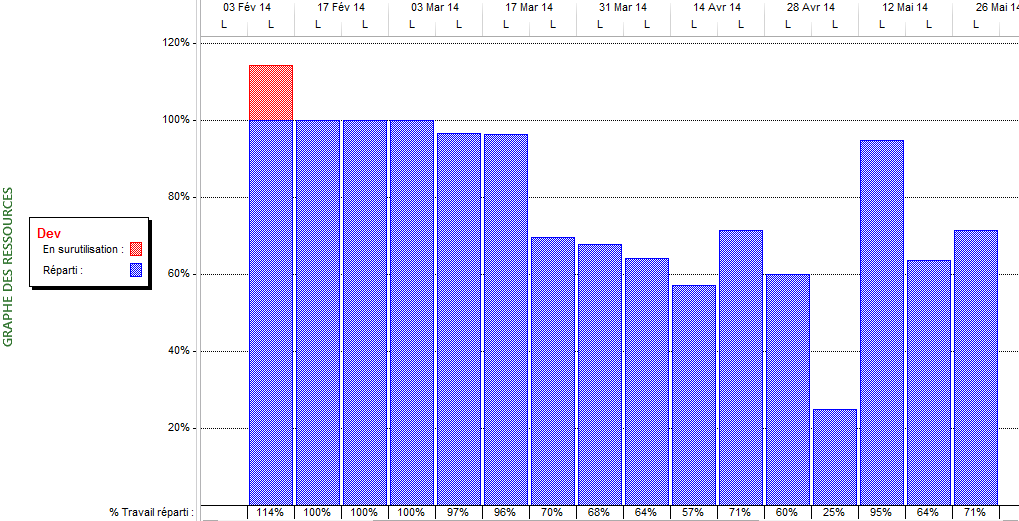
\includegraphics[width=1.5\textwidth, angle=90]{UtilisationDesRessources.png}

\caption{\label{fig:sample-graph}Diagramme de taux d'utilisation des ressources}
\end{figure}




\chapter{Conclusion}

Le tableau ci-dessous récapitule la planification du projet selon les tâches principales à effectuer:

\begin{table}[H]
\centering
  \begin{tabularx}{0.8\textwidth}{| X | c |}
    \hline
	Tâches & Charges \\
    \hline
    Conception & 40h \\
    Développement & 375h \\
    Tests & 60h \\
    Rapport final & 40h \\
    Préaparation de la soutenance & 20h \\
    \hline
	Total & 535h \\
    \hline
  \end{tabularx}
  \caption{Durées des tâches principales}
\end{table}

Dans ce document, nous avons estimé dans la mesure du possible, selon nos connaissances et notre réflexion, les durées en heures relatives à chaque étape. Ces évaluations seront peut être amenées à être modifiées au fûr et à mesure de l'avancée du projet.
Avant de pouvoir commencer le développement, nous allons concevoir l'architecture interne du logiciel et modéliser les différentes interactions entre les différents modules. Cette prochaine étape sera l'objet du rapport de conception logicielle.


\end{document}